% Options for packages loaded elsewhere
\PassOptionsToPackage{unicode}{hyperref}
\PassOptionsToPackage{hyphens}{url}
%
\documentclass[
]{article}
\usepackage{amsmath,amssymb}
\usepackage{iftex}
\ifPDFTeX
  \usepackage[T1]{fontenc}
  \usepackage[utf8]{inputenc}
  \usepackage{textcomp} % provide euro and other symbols
\else % if luatex or xetex
  \usepackage{unicode-math} % this also loads fontspec
  \defaultfontfeatures{Scale=MatchLowercase}
  \defaultfontfeatures[\rmfamily]{Ligatures=TeX,Scale=1}
\fi
\usepackage{lmodern}
\ifPDFTeX\else
  % xetex/luatex font selection
\fi
% Use upquote if available, for straight quotes in verbatim environments
\IfFileExists{upquote.sty}{\usepackage{upquote}}{}
\IfFileExists{microtype.sty}{% use microtype if available
  \usepackage[]{microtype}
  \UseMicrotypeSet[protrusion]{basicmath} % disable protrusion for tt fonts
}{}
\makeatletter
\@ifundefined{KOMAClassName}{% if non-KOMA class
  \IfFileExists{parskip.sty}{%
    \usepackage{parskip}
  }{% else
    \setlength{\parindent}{0pt}
    \setlength{\parskip}{6pt plus 2pt minus 1pt}}
}{% if KOMA class
  \KOMAoptions{parskip=half}}
\makeatother
\usepackage{xcolor}
\usepackage[margin=1in]{geometry}
\usepackage{color}
\usepackage{fancyvrb}
\newcommand{\VerbBar}{|}
\newcommand{\VERB}{\Verb[commandchars=\\\{\}]}
\DefineVerbatimEnvironment{Highlighting}{Verbatim}{commandchars=\\\{\}}
% Add ',fontsize=\small' for more characters per line
\usepackage{framed}
\definecolor{shadecolor}{RGB}{248,248,248}
\newenvironment{Shaded}{\begin{snugshade}}{\end{snugshade}}
\newcommand{\AlertTok}[1]{\textcolor[rgb]{0.94,0.16,0.16}{#1}}
\newcommand{\AnnotationTok}[1]{\textcolor[rgb]{0.56,0.35,0.01}{\textbf{\textit{#1}}}}
\newcommand{\AttributeTok}[1]{\textcolor[rgb]{0.13,0.29,0.53}{#1}}
\newcommand{\BaseNTok}[1]{\textcolor[rgb]{0.00,0.00,0.81}{#1}}
\newcommand{\BuiltInTok}[1]{#1}
\newcommand{\CharTok}[1]{\textcolor[rgb]{0.31,0.60,0.02}{#1}}
\newcommand{\CommentTok}[1]{\textcolor[rgb]{0.56,0.35,0.01}{\textit{#1}}}
\newcommand{\CommentVarTok}[1]{\textcolor[rgb]{0.56,0.35,0.01}{\textbf{\textit{#1}}}}
\newcommand{\ConstantTok}[1]{\textcolor[rgb]{0.56,0.35,0.01}{#1}}
\newcommand{\ControlFlowTok}[1]{\textcolor[rgb]{0.13,0.29,0.53}{\textbf{#1}}}
\newcommand{\DataTypeTok}[1]{\textcolor[rgb]{0.13,0.29,0.53}{#1}}
\newcommand{\DecValTok}[1]{\textcolor[rgb]{0.00,0.00,0.81}{#1}}
\newcommand{\DocumentationTok}[1]{\textcolor[rgb]{0.56,0.35,0.01}{\textbf{\textit{#1}}}}
\newcommand{\ErrorTok}[1]{\textcolor[rgb]{0.64,0.00,0.00}{\textbf{#1}}}
\newcommand{\ExtensionTok}[1]{#1}
\newcommand{\FloatTok}[1]{\textcolor[rgb]{0.00,0.00,0.81}{#1}}
\newcommand{\FunctionTok}[1]{\textcolor[rgb]{0.13,0.29,0.53}{\textbf{#1}}}
\newcommand{\ImportTok}[1]{#1}
\newcommand{\InformationTok}[1]{\textcolor[rgb]{0.56,0.35,0.01}{\textbf{\textit{#1}}}}
\newcommand{\KeywordTok}[1]{\textcolor[rgb]{0.13,0.29,0.53}{\textbf{#1}}}
\newcommand{\NormalTok}[1]{#1}
\newcommand{\OperatorTok}[1]{\textcolor[rgb]{0.81,0.36,0.00}{\textbf{#1}}}
\newcommand{\OtherTok}[1]{\textcolor[rgb]{0.56,0.35,0.01}{#1}}
\newcommand{\PreprocessorTok}[1]{\textcolor[rgb]{0.56,0.35,0.01}{\textit{#1}}}
\newcommand{\RegionMarkerTok}[1]{#1}
\newcommand{\SpecialCharTok}[1]{\textcolor[rgb]{0.81,0.36,0.00}{\textbf{#1}}}
\newcommand{\SpecialStringTok}[1]{\textcolor[rgb]{0.31,0.60,0.02}{#1}}
\newcommand{\StringTok}[1]{\textcolor[rgb]{0.31,0.60,0.02}{#1}}
\newcommand{\VariableTok}[1]{\textcolor[rgb]{0.00,0.00,0.00}{#1}}
\newcommand{\VerbatimStringTok}[1]{\textcolor[rgb]{0.31,0.60,0.02}{#1}}
\newcommand{\WarningTok}[1]{\textcolor[rgb]{0.56,0.35,0.01}{\textbf{\textit{#1}}}}
\usepackage{graphicx}
\makeatletter
\def\maxwidth{\ifdim\Gin@nat@width>\linewidth\linewidth\else\Gin@nat@width\fi}
\def\maxheight{\ifdim\Gin@nat@height>\textheight\textheight\else\Gin@nat@height\fi}
\makeatother
% Scale images if necessary, so that they will not overflow the page
% margins by default, and it is still possible to overwrite the defaults
% using explicit options in \includegraphics[width, height, ...]{}
\setkeys{Gin}{width=\maxwidth,height=\maxheight,keepaspectratio}
% Set default figure placement to htbp
\makeatletter
\def\fps@figure{htbp}
\makeatother
\setlength{\emergencystretch}{3em} % prevent overfull lines
\providecommand{\tightlist}{%
  \setlength{\itemsep}{0pt}\setlength{\parskip}{0pt}}
\setcounter{secnumdepth}{-\maxdimen} % remove section numbering
\ifLuaTeX
  \usepackage{selnolig}  % disable illegal ligatures
\fi
\usepackage{bookmark}
\IfFileExists{xurl.sty}{\usepackage{xurl}}{} % add URL line breaks if available
\urlstyle{same}
\hypersetup{
  pdftitle={Shiny Apps in R},
  pdfauthor={Matt Hewitt},
  hidelinks,
  pdfcreator={LaTeX via pandoc}}

\title{Shiny Apps in R}
\author{Matt Hewitt}
\date{2024-08-21}

\begin{document}
\maketitle

\section{Shiny Structure}\label{shiny-structure}

Shiny apps will all have the same 3 parts, some may have MUCH more, but
all will have these three basic parts.

\subsubsection{Global}\label{global}

This part of the app is intended for you to `get things set up'. This is
where you would load all the necessary packages, load data, connect to
databases, source other files/scripts, any any other pieces of
information your app needs to operate. This is usually not needed for
simple apps, but can be extensive in larger ones.

\subsubsection{UI (User Interface)}\label{ui-user-interface}

This is the portion of the app that the user actually sees and interacts
with. It can be as specific or as general as needed, usually very
specific for basic apps and general for more complicated ones. If you do
not need things in the UI to change while the app is being used, all UI
structure can be built in the UI portion of the code. However; if the
presence of things, such as drop down menus or tables, is dependent on
inputs from the user, then that portion of the UI will end up being
built in the Server portion of the code.

There are many packages that provide pre-built layouts, my favorite is
shiny dashboard. Think of it as base R graphics and ggplot2, the base
graphics work, but ggplot tends to be a lot prettier and more flexible.
Shiny dashboard has some great resources for helping you build intuitive
and aesthetically pleasing UI's
(\url{https://rstudio.github.io/shinydashboard/}).

There is a structured way that UI's are built. We will use the
\texttt{sidebarLayout()} layout further down in this document. Here are
some examples of shiny's default layouts:\\

\begin{figure}
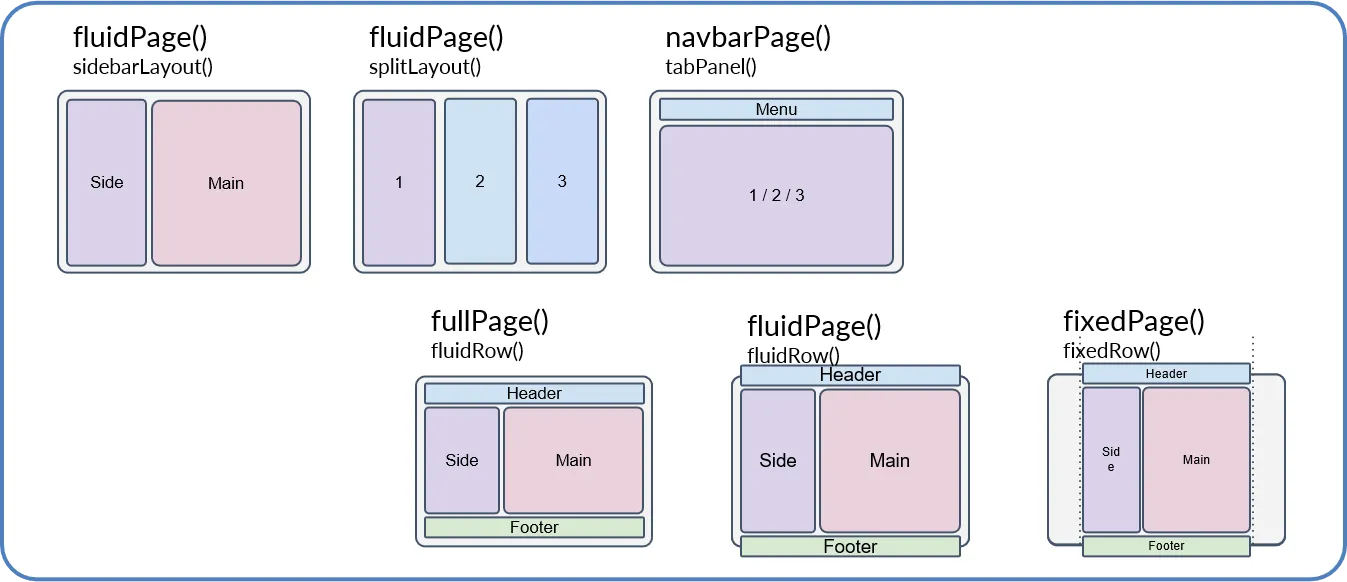
\includegraphics[width=700px,height=300]{figures/shiny-layouts} \caption{A nice image.}\label{fig:unnamed-chunk-1}
\end{figure}

\hfill\break

Within the sections of these layouts (or just a blank page, if you
choose to go that route) there is a structure for placing items on the
page. Items include anything, user inputs, outputs, tables, figures,
boxes, titles, literally anything you want to place on the page. The
method for `mapping' where items are placed follow this structure:\\

\begin{figure}
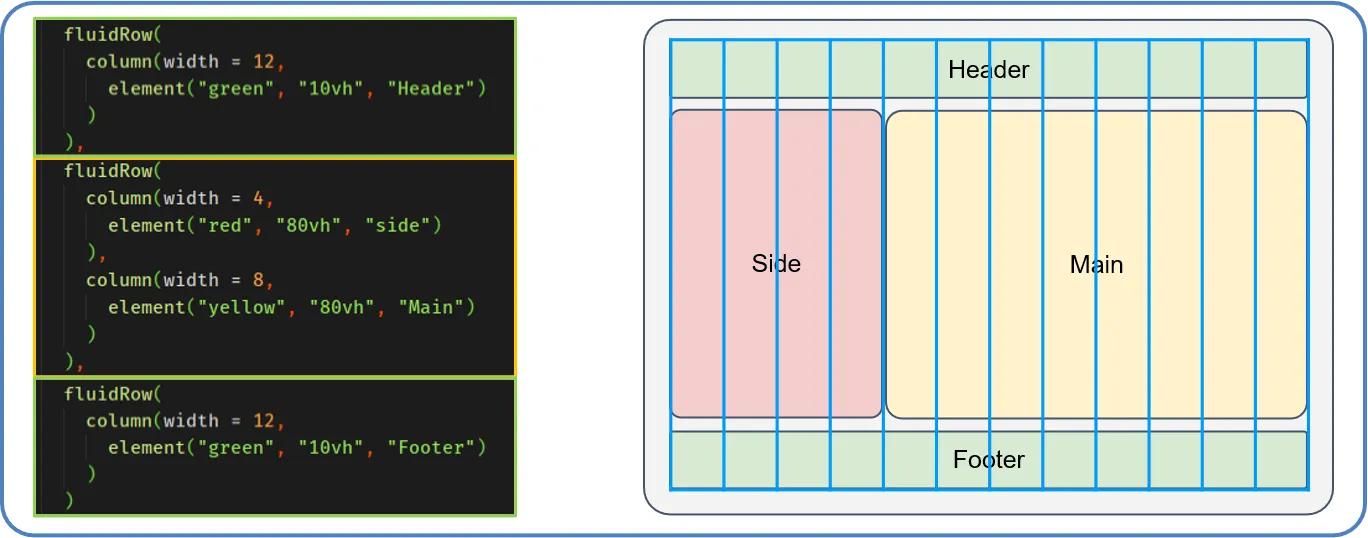
\includegraphics[width=700px,height=300]{figures/bootstrap-layout} \caption{A nice image.}\label{fig:unnamed-chunk-2}
\end{figure}

This graphic is a custom made layout, not one of the preset layouts
through shiny. The three sections in the R code on the left side (the
three \texttt{fluidRow()}'s) correspond to the three rows on the example
layout on the right (the Header, Side/Main, and Footer). The first
\texttt{fluidRow()} that creates the Header section contains a
\texttt{column()} function. Just as the names would suggest,
\texttt{fluidRow()} creates rows, and \texttt{column()} creates columns.
Because \texttt{column()} is nested within \texttt{fluidRow()} in this
instance, it will create a single column of width 12 within the Header
section. It is within \texttt{column()} that you would place elements to
have them be displayed within the Header section.

You can see the center portion of the code has two \texttt{column()}'s
within the \texttt{fluidRow()}. These correspond to the Side and Main
portions of the layout on the right. The first \texttt{column()} is of
width 4, and the second \texttt{column()} is of width 8, which add up to
the total width of 12 to fill the width of the page. It isn't shown
explicitly in this figure, but the width of each section is 12. So even
though the Side section is only of with 4 when looking at the entire
page, when we start placing elements within the section, we have a width
of 12 to work with again.

The height of the different sections is dictated by what elements you
place within each \texttt{column()}. If you ran this example code here,
all three \texttt{fluidRow()}'s would be the same height.

\subsubsection{Server}\label{server}

This is where the magic happens! The \textbf{Server} file is where all
processes and operations live that dictate the behavior of your app. The
app will continuously be observing the server file and will run its
different portions given different user inputs.

There are two parts, essentially list objects, that live underneath the
operations of the server; the input and output. The input object is
where all element input values live. Examples of input elements are
\texttt{textInput()}, \texttt{selectInput()}, \texttt{actionButton()},
\texttt{numericInput()}, and \texttt{dateInput()}. These are very handy
input functions that create elements users can interact with to input
data.

When you create an element in the \textbf{UI} (or wherever you create
the element) you assign it an inputid. This id, or tag, will be how you
access the value of, or make functions observe, different input
elements.

A major part of how shiny operates is by \emph{observing} different
portions of the \textbf{Server} file. There are many functions that
dictate how this works, but some of the most common ones are
\texttt{observe()} and \texttt{observeEvent()}. The \texttt{observe()}
function tells R to continuously run the code within it. I don't
entirely understand how R knows when or how often to run all the
\texttt{observe()} functions within the \textbf{Server} file, but
somehow it gets it right. The code within \texttt{observeEvent()}
functions will only be run when a specific event happens.

\newpage

\subsection{Shiny Function}\label{shiny-function}

The App will run these pieces in a particular order. It will start with
the \textbf{Global} portion, then the \textbf{UI}, and lastly the
\textbf{Server}. The \textbf{Global} and \textbf{UI} will only be run
once, when the app start up, but the server will constantly be observed
and portions will be re-run given inputs from the user.

Lets look at a basic app. The following is the default example present
in every new shiny file:

\begin{Shaded}
\begin{Highlighting}[]
    \DocumentationTok{\#\# Global {-}{-}{-}{-}{-}{-}{-}{-}{-}{-}{-}{-}{-}{-}{-}{-}{-}{-}{-}{-}{-}{-}{-}{-}{-}{-}{-}{-}{-}{-}{-}{-}{-}{-}{-}{-}{-}{-}{-}{-}{-}{-}{-}{-}{-}{-}{-}{-}{-}{-} Load packages}
\FunctionTok{library}\NormalTok{(shiny)}

    \DocumentationTok{\#\# UI {-}{-}{-}{-}{-}{-}{-}{-}{-}{-}{-}{-}{-}{-}{-}{-}{-}{-}{-}{-}{-}{-}{-}{-}{-}{-}{-}{-}{-}{-}{-}{-}{-}{-}{-}{-}{-}{-}{-}{-}{-}{-}{-}{-}{-}{-}{-}{-}{-}{-}{-}{-}{-}{-} Create User Interface layout}
\NormalTok{ui }\OtherTok{\textless{}{-}} \FunctionTok{fluidPage}\NormalTok{(}

    \CommentTok{\# Application title}
    \FunctionTok{titlePanel}\NormalTok{(}\StringTok{"Old Faithful Geyser Data"}\NormalTok{),}

    \CommentTok{\# Sidebar with a slider input for number of bins }
    \FunctionTok{sidebarLayout}\NormalTok{(}
        \FunctionTok{sidebarPanel}\NormalTok{(}
            \FunctionTok{sliderInput}\NormalTok{(}\StringTok{"bins"}\NormalTok{,}
                        \StringTok{"Number of bins:"}\NormalTok{,}
                        \AttributeTok{min =} \DecValTok{1}\NormalTok{,}
                        \AttributeTok{max =} \DecValTok{50}\NormalTok{,}
                        \AttributeTok{value =} \DecValTok{30}\NormalTok{)}
\NormalTok{        ),}

        \CommentTok{\# Show a plot of the generated distribution}
        \FunctionTok{mainPanel}\NormalTok{(}
           \FunctionTok{plotOutput}\NormalTok{(}\StringTok{"distPlot"}\NormalTok{)}
\NormalTok{        )}
\NormalTok{    )}
\NormalTok{)}

    \DocumentationTok{\#\# Server {-}{-}{-}{-}{-}{-}{-}{-}{-}{-}{-}{-}{-}{-}{-}{-}{-}{-}{-}{-}{-}{-}{-}{-}{-}{-}{-}{-}{-}{-}{-}{-}{-}{-}{-}{-}{-}{-}{-}{-}{-}{-}{-}{-}{-}{-}{-}{-}{-}{-} Define Server logic}
\NormalTok{server }\OtherTok{\textless{}{-}} \ControlFlowTok{function}\NormalTok{(input, output) \{}

\NormalTok{    output}\SpecialCharTok{$}\NormalTok{distPlot }\OtherTok{\textless{}{-}} \FunctionTok{renderPlot}\NormalTok{(\{}
        \CommentTok{\# generate bins based on input$bins from ui.R}
\NormalTok{        x    }\OtherTok{\textless{}{-}}\NormalTok{ faithful[, }\DecValTok{2}\NormalTok{]}
\NormalTok{        bins }\OtherTok{\textless{}{-}} \FunctionTok{seq}\NormalTok{(}\FunctionTok{min}\NormalTok{(x), }\FunctionTok{max}\NormalTok{(x), }\AttributeTok{length.out =}\NormalTok{ input}\SpecialCharTok{$}\NormalTok{bins }\SpecialCharTok{+} \DecValTok{1}\NormalTok{)}

        \CommentTok{\# draw the histogram with the specified number of bins}
        \FunctionTok{hist}\NormalTok{(x, }\AttributeTok{breaks =}\NormalTok{ bins, }\AttributeTok{col =} \StringTok{\textquotesingle{}darkgray\textquotesingle{}}\NormalTok{, }\AttributeTok{border =} \StringTok{\textquotesingle{}white\textquotesingle{}}\NormalTok{,}
             \AttributeTok{xlab =} \StringTok{\textquotesingle{}Waiting time to next eruption (in mins)\textquotesingle{}}\NormalTok{,}
             \AttributeTok{main =} \StringTok{\textquotesingle{}Histogram of waiting times\textquotesingle{}}\NormalTok{)}
\NormalTok{    \})}
\NormalTok{\}}

    \DocumentationTok{\#\# {-}{-}{-}{-}{-}{-}{-}{-}{-}{-}{-}{-}{-}{-}{-}{-}{-}{-}{-}{-}{-}{-}{-}{-}{-}{-}{-}{-}{-}{-}{-}{-}{-}{-}{-}{-}{-}{-}{-}{-}{-}{-}{-}{-}{-}{-}{-}{-}{-}{-}{-}{-}{-}{-}{-}{-}{-} Run the application }
\FunctionTok{shinyApp}\NormalTok{(}\AttributeTok{ui =}\NormalTok{ ui, }\AttributeTok{server =}\NormalTok{ server)}
\end{Highlighting}
\end{Shaded}

In this app you can see the 3 basic parts. This particular app is a `one
file' app. Meaning all portions of the application are housed in one
file. Alternatively, you can split all the portions of this up into
different files. Meaning, your \textbf{Global}, \textbf{UI} and
\textbf{Server} portions will all be in their own .R file.

But, we will continue with the single file format for now to keep things
simple.

The \textbf{Global} portion of this app is super simple, we are just
loading the `shiny' package into our environment.

The \textbf{UI} portion here actually has a little ore going on. As you
can see, this portion is just one big function called
\texttt{fluidPage()} with a few other things happening inside. The
visual portion of shiny is all based off HTML, the coding language used
to build websites. If you are curious, right click on any webpage and
hit the `inspect' button in the menu and it will show you all the
underlying HTML. It's really gross!! Shiny is cool because it allows you
to wrangle the flexibility and power of HTML, without needing to know
how to code in HTML. Shiny provides you with a surprisingly
comprehensive set of functions that build HTML layouts as a result so
you don't have to. Phew!!

So, lets break down whats happening in the \texttt{fluidPage()}
function. There are many nested function within it, but the next
immediate level down is \texttt{sidebarlayout()}. This is one of the
pre-packaged base shiny layouts that has a side bar and main body areas
we saw above. The two functions at the next level down are
\texttt{sidebarPanel()} and \texttt{mainPanel()}. This is where you tell
R what you want to put into each of these areas. In
\texttt{sidebarPanel()} we have a \texttt{sliderInput()}, which creates
a slider bar the user can move back and forth that we internally labeled
as `bins' (I'll explain what that means in a bit), gave it a title to
display above the slider bar `Number of bins:', restricted the values
between 1 and 50, and set the initial value to 30. Inside the
\texttt{mainPanel()} function we have \texttt{plotOutput()}, which,
unlike an input function, just creates a spot something can be put
later. In this case, this spot will only accept a plot. We internally
labeled this currently unoccupied spot `distPlot'.

If we run this code, because it is a single file type app and it is
already structured properly, things will run from top to bottom.
Starting with loading the package.

\end{document}
